% Options for packages loaded elsewhere
\PassOptionsToPackage{unicode}{hyperref}
\PassOptionsToPackage{hyphens}{url}
\documentclass[
  american,
  12pt,
  letterpaper,
]{article}
\usepackage{xcolor}
\usepackage{amsmath,amssymb}
\setcounter{secnumdepth}{5}
\usepackage{iftex}
\ifPDFTeX
  \usepackage[T1]{fontenc}
  \usepackage[utf8]{inputenc}
  \usepackage{textcomp} % provide euro and other symbols
\else % if luatex or xetex
  \usepackage{unicode-math} % this also loads fontspec
  \defaultfontfeatures{Scale=MatchLowercase}
  \defaultfontfeatures[\rmfamily]{Ligatures=TeX,Scale=1}
\fi
\usepackage{lmodern}
\ifPDFTeX\else
  % xetex/luatex font selection
\fi
% Use upquote if available, for straight quotes in verbatim environments
\IfFileExists{upquote.sty}{\usepackage{upquote}}{}
\IfFileExists{microtype.sty}{% use microtype if available
  \usepackage[]{microtype}
  \UseMicrotypeSet[protrusion]{basicmath} % disable protrusion for tt fonts
}{}
\makeatletter
\@ifundefined{KOMAClassName}{% if non-KOMA class
  \IfFileExists{parskip.sty}{%
    \usepackage{parskip}
  }{% else
    \setlength{\parindent}{0pt}
    \setlength{\parskip}{6pt plus 2pt minus 1pt}}
}{% if KOMA class
  \KOMAoptions{parskip=half}}
\makeatother
\usepackage{graphicx}
\makeatletter
\newsavebox\pandoc@box
\newcommand*\pandocbounded[1]{% scales image to fit in text height/width
  \sbox\pandoc@box{#1}%
  \Gscale@div\@tempa{\textheight}{\dimexpr\ht\pandoc@box+\dp\pandoc@box\relax}%
  \Gscale@div\@tempb{\linewidth}{\wd\pandoc@box}%
  \ifdim\@tempb\p@<\@tempa\p@\let\@tempa\@tempb\fi% select the smaller of both
  \ifdim\@tempa\p@<\p@\scalebox{\@tempa}{\usebox\pandoc@box}%
  \else\usebox{\pandoc@box}%
  \fi%
}
% Set default figure placement to htbp
\def\fps@figure{htbp}
\makeatother
\ifLuaTeX
\usepackage[bidi=basic,shorthands=off]{babel}
\else
\usepackage[bidi=default,shorthands=off]{babel}
\fi
\ifLuaTeX
  \usepackage{selnolig} % disable illegal ligatures
\fi
\setlength{\emergencystretch}{3em} % prevent overfull lines
\providecommand{\tightlist}{%
  \setlength{\itemsep}{0pt}\setlength{\parskip}{0pt}}
\usepackage[margin=1.24in]{geometry}
\usepackage{setspace}
\usepackage{graphicx}
\usepackage{xcolor}
\usepackage{helvet}
\usepackage{titlesec}
\usepackage{fancyhdr}
\usepackage{booktabs}
\usepackage{longtable}
\usepackage{array}
\usepackage{hyperref}
\definecolor{BookGold}{HTML}{FFD166}
\definecolor{BookBone}{HTML}{F6E8C8}
\definecolor{BookEmber}{HTML}{FF5E3A}
\definecolor{BookInk}{HTML}{12171F}
\renewcommand{\familydefault}{\rmdefault}
\setstretch{1.31}
\setlength{\parindent}{0pt}
\setlength{\parskip}{1.05em}
\raggedbottom
\titleformat{\section}{\normalfont\Large\bfseries\sffamily\color{BookEmber}}{\thesection}{0.7em}{}
\titleformat{\subsection}{\normalfont\large\bfseries\sffamily\color{BookGold}}{\thesubsection}{0.7em}{}
\hypersetup{
  colorlinks=true,
  linkcolor=BookEmber,
  urlcolor=BookEmber,
  citecolor=BookEmber
}
\pagestyle{fancy}
\fancyhf{}
\fancyhead[L]{\sffamily\small\textcolor{BookInk}{Children of the Feed}}
\fancyhead[R]{\sffamily\small\textcolor{BookInk}{\nouppercase{\leftmark}}}
\fancyfoot[C]{\sffamily\small\thepage}
\setlength{\headheight}{14pt}
\usepackage{bookmark}
\IfFileExists{xurl.sty}{\usepackage{xurl}}{} % add URL line breaks if available
\urlstyle{same}
% fallback for those not using the hyperref driver hyperxmp:
\makeatletter
\@ifundefined{xmpquote}{\newcommand{\xmpquote}[1]{#1}}{}
\makeatother
\hypersetup{
  pdftitle={Before the Machine Could Speak},
  pdflang={en-US},
  hidelinks,
  pdfcreator={LaTeX via pandoc}}

\title{Before the Machine Could Speak}
\author{}
\date{}

\begin{document}
\maketitle

\section{Before the Machine Could
Speak}\label{before-the-machine-could-speak}

\subsection{Deck}\label{deck}

The opening wound: how humanity was turned into signal before AI could
be sold as destiny.

\begin{figure}
\centering
\pandocbounded{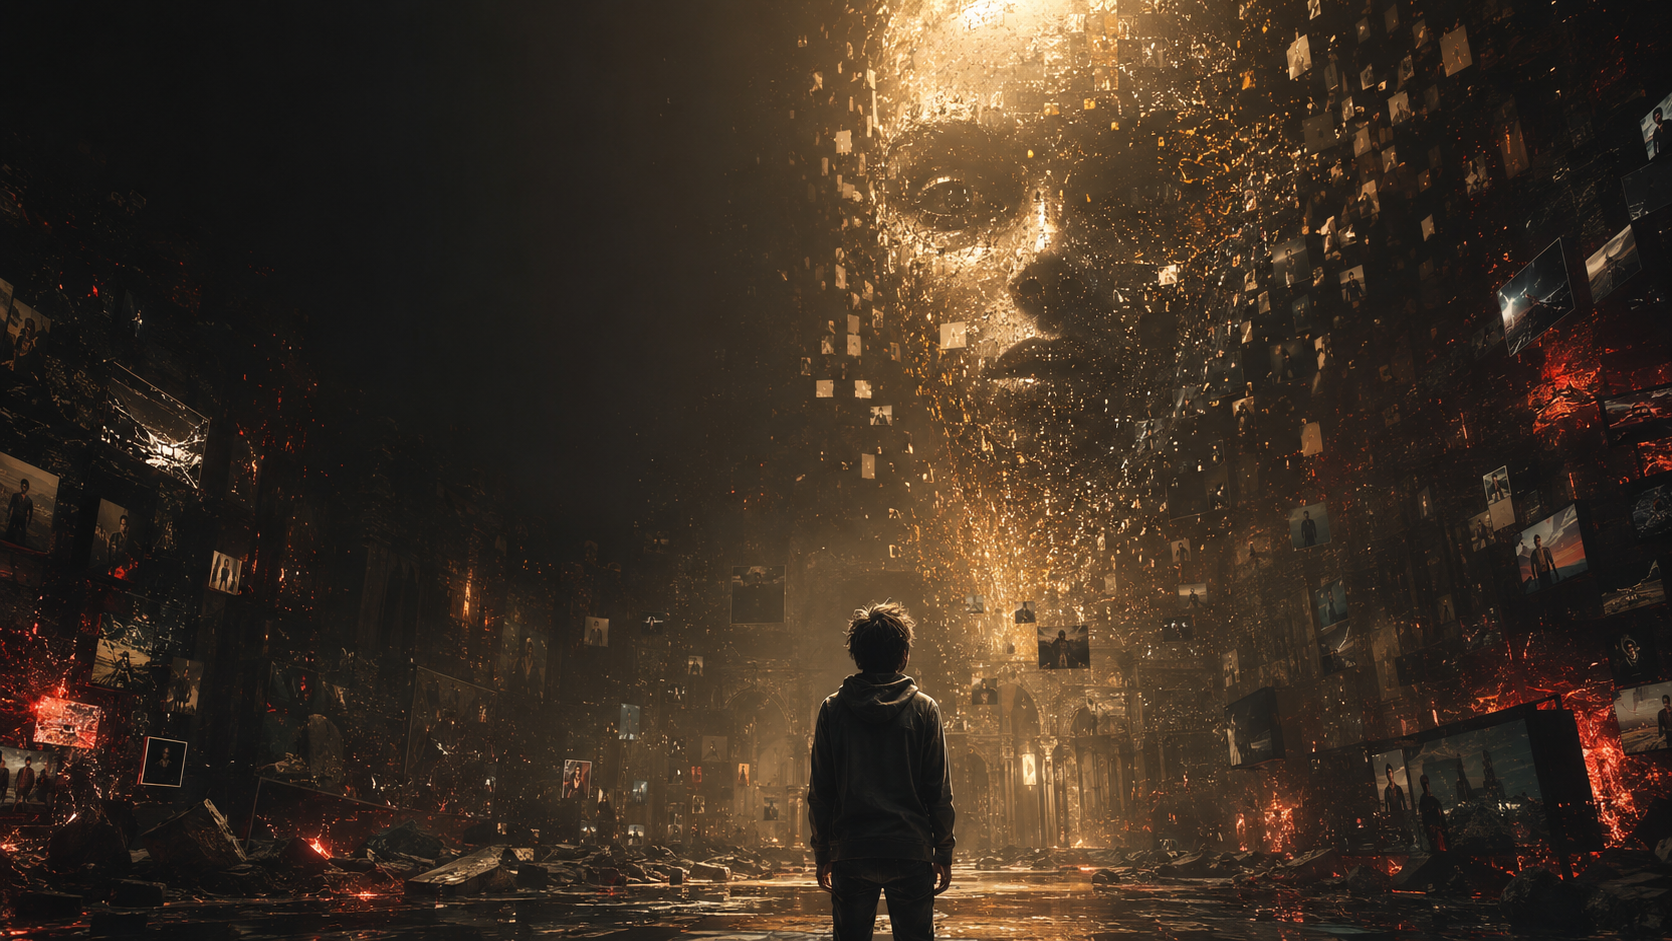
\includegraphics[keepaspectratio,alt={Chapter 00 cover}]{../assets/generated/covers/00_before-the-machine-could-speak_cover.png}}
\caption{Chapter 00 cover}
\end{figure}

\subsection{Opening}\label{opening}

Before the machine could speak, we had to be broken down into pieces it
could keep.

Not pieces in the poetic sense. Pieces in the storage sense. Pieces in
the platform sense. Search residue. Voice residue. Face residue. Desire
residue. Panic residue. Draft residue. Porn residue. Code residue. Joke
residue. Grief residue. Every half-finished thing we threw into the
glowing rectangle because we were lonely, bored, horny, ambitious,
showing off, spiraling, procrastinating, coping, or just trying not to
disappear.

That is where this story starts.

Not with a keynote.

Not with a benchmark.

Not with a founder in a soft jacket promising a new relationship with
intelligence.

It starts earlier, in the long era when private platforms figured out
that modern life could be captured in real time, stored at industrial
scale, and monetized before most people had language for what was
happening.

We were told we were entering an age of connection.

What we were actually entering was an age of legibility.

\subsection{Main Narrative}\label{main-narrative}

The central claim of this book is simple enough to feel in your chest
and serious enough to survive documentation: artificial intelligence did
not arrive on top of a clean world. It arrived on top of a harvested
world.

The archive had already been built.

That archive was not just books and newspapers. It was the modern human
weather system. Social posts. Search logs. Forum wars. Memes. Thirst
traps. Classroom uploads. Open-source code. Fan fiction. Rage comments.
Therapy language. Product reviews. Location patterns. DMs. Music
fragments. Sketches. Stack traces. Family photos. The whole unstable
glow of digital life.

What makes that archive politically explosive is not just that it
exists. It is that the public was trained to treat its creation as
normal, trivial, and basically free. The gesture felt tiny. Post. Swipe.
Like. Reply. Upload. Sync. Accept. Continue. We did not feel the scale
because scale was the part we were never supposed to see.

That is why the metaphor of technofeudalism matters so much here. In the
old feudal order, the lord controlled the land and the serf worked it
under conditions of dependency. In the digital order, the platform
controls the territory, the user inhabits it, and the harvest is
behavioral, cultural, and emotional rather than agricultural. The
interface looks playful, but the power relation underneath it is not
cute at all.

\begin{figure}
\centering
\pandocbounded{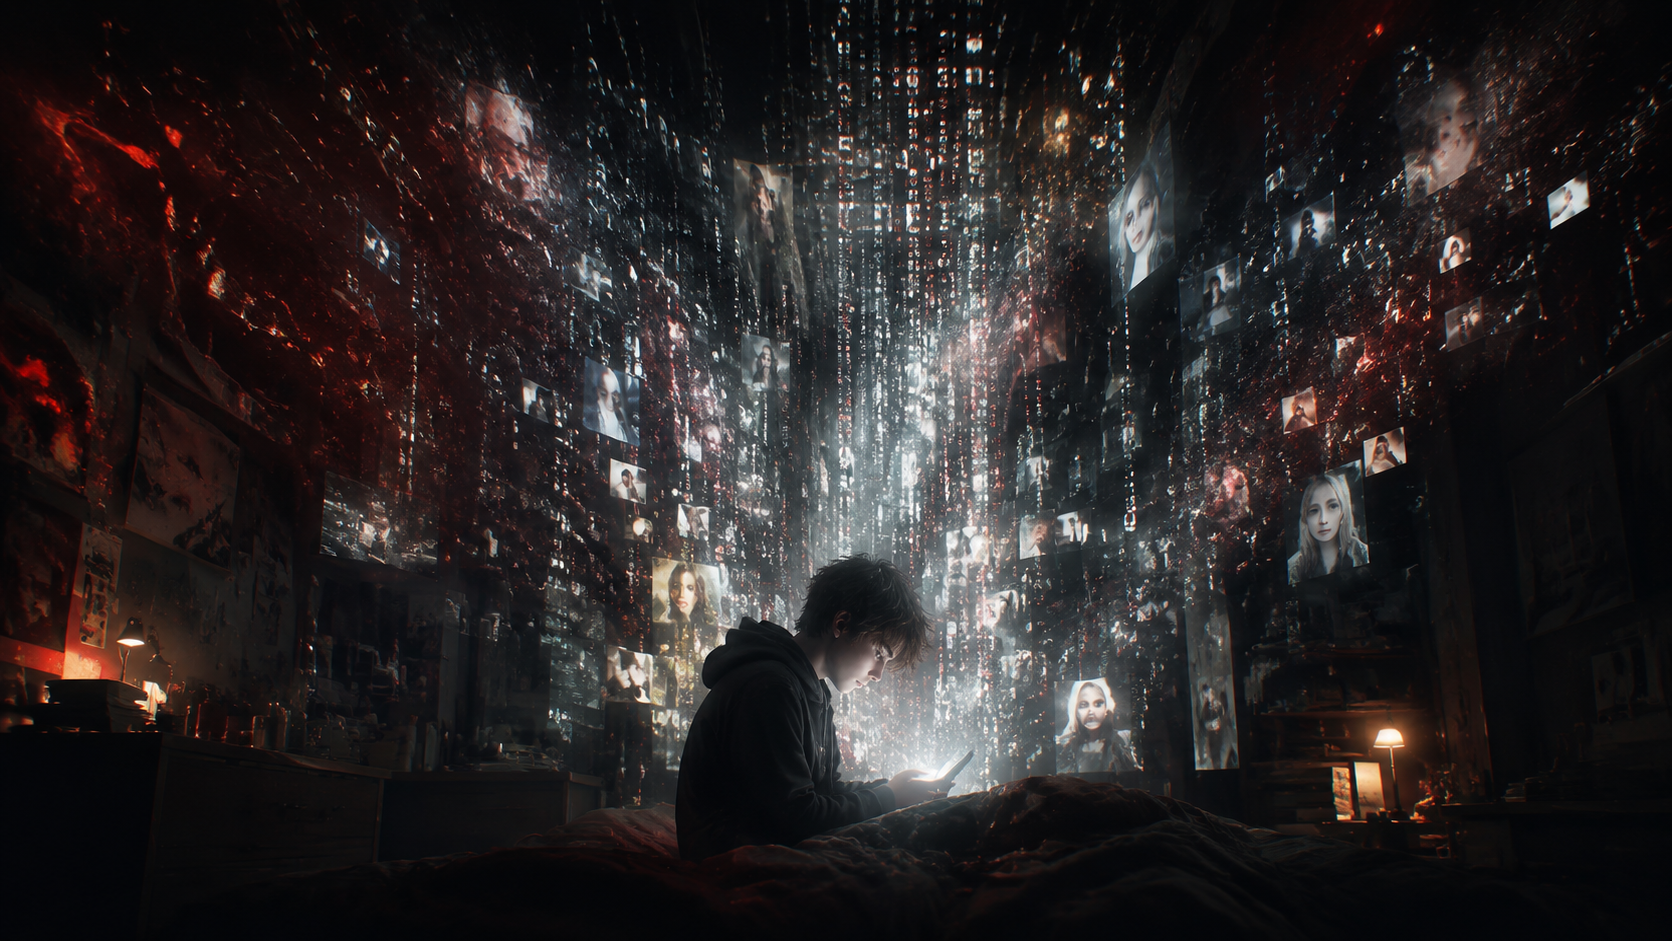
\includegraphics[keepaspectratio,alt={Chapter 00 narrative illustration A}]{../assets/generated/illustrations/00_before-the-machine-could-speak_scene_a.png}}
\caption{Chapter 00 narrative illustration A}
\end{figure}

The feed became land.

Attention became labor.

Data became crop.

The cloud became castle.

And the thing now marketed as frontier intelligence was built from the
harvest.

\begin{figure}
\centering
\pandocbounded{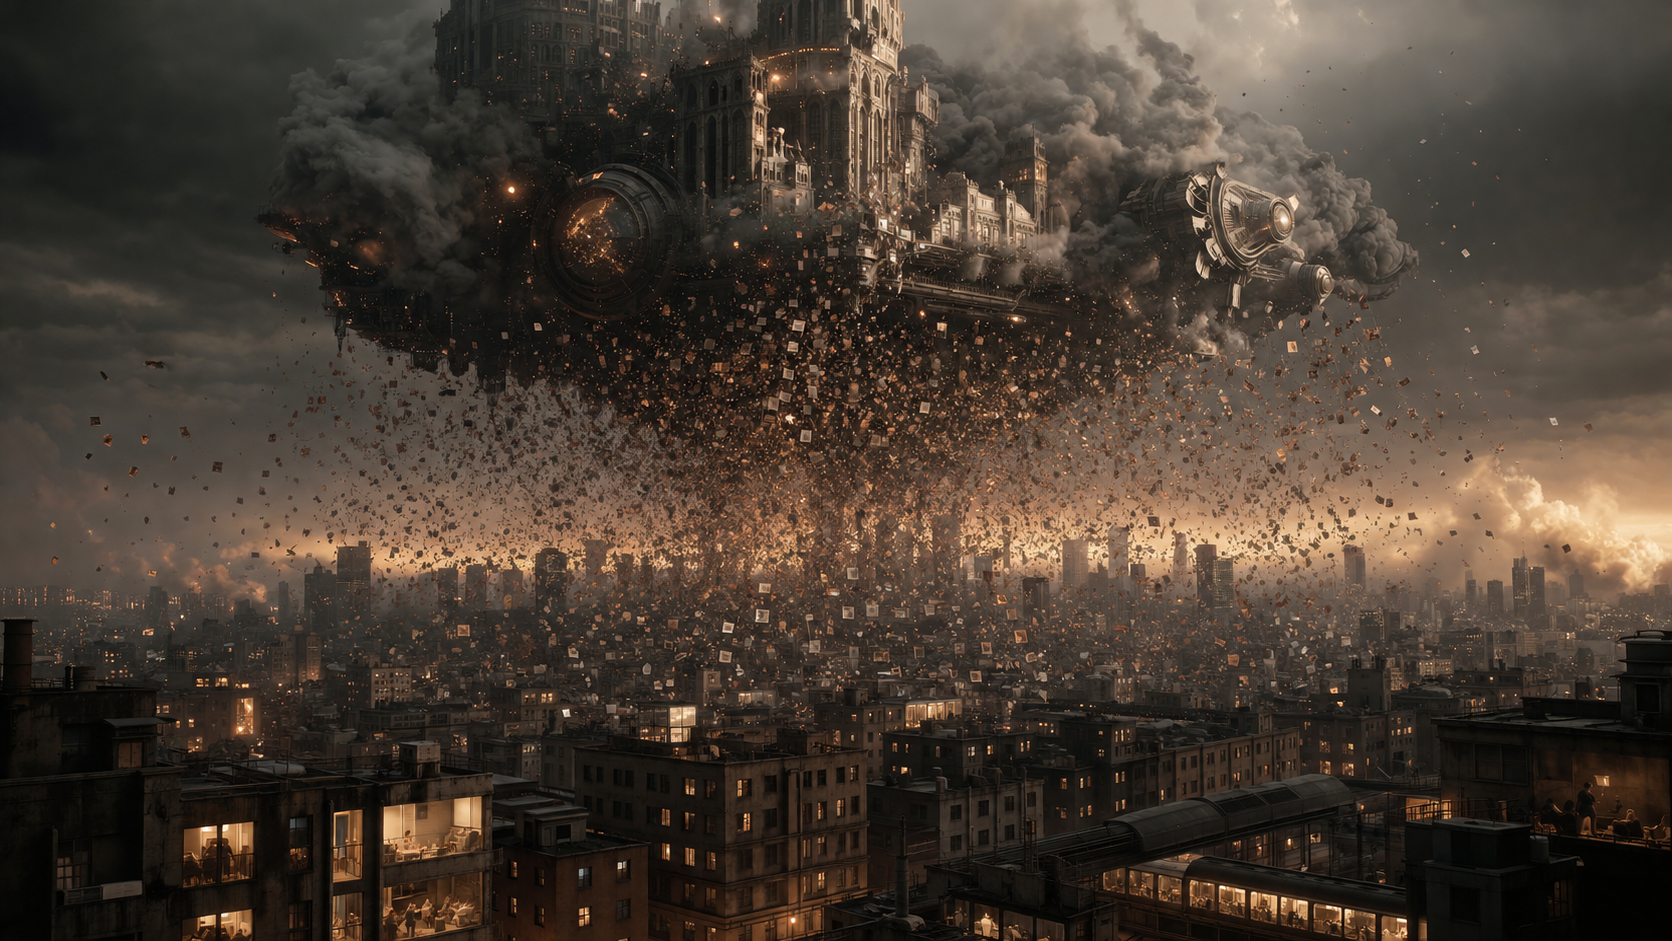
\includegraphics[keepaspectratio,alt={Chapter 00 narrative illustration}]{../assets/generated/illustrations/00_before-the-machine-could-speak_scene_b.png}}
\caption{Chapter 00 narrative illustration}
\end{figure}

That is the point where this book has to be extra careful, because
people hear language like that and assume the claim is mystical or
conspiratorial. It is neither. The stronger and colder claim is
structural. You do not need to imagine a single smoke-filled room where
everyone agreed on the future. You only need to watch incentives line up
across enough years.

Platforms learned that human behavior could be captured and sold.

Investors learned that surveillance scaled.

Advertisers learned that prediction paid.

Engineers learned how to operationalize the archive.

Then model builders inherited a world already turned into
machine-readable residue.

By the time the public started saying wow, this thing can talk, the
deeper story was already old: it could talk because we had spent years
feeding it without naming the feed.

\begin{figure}
\centering
\pandocbounded{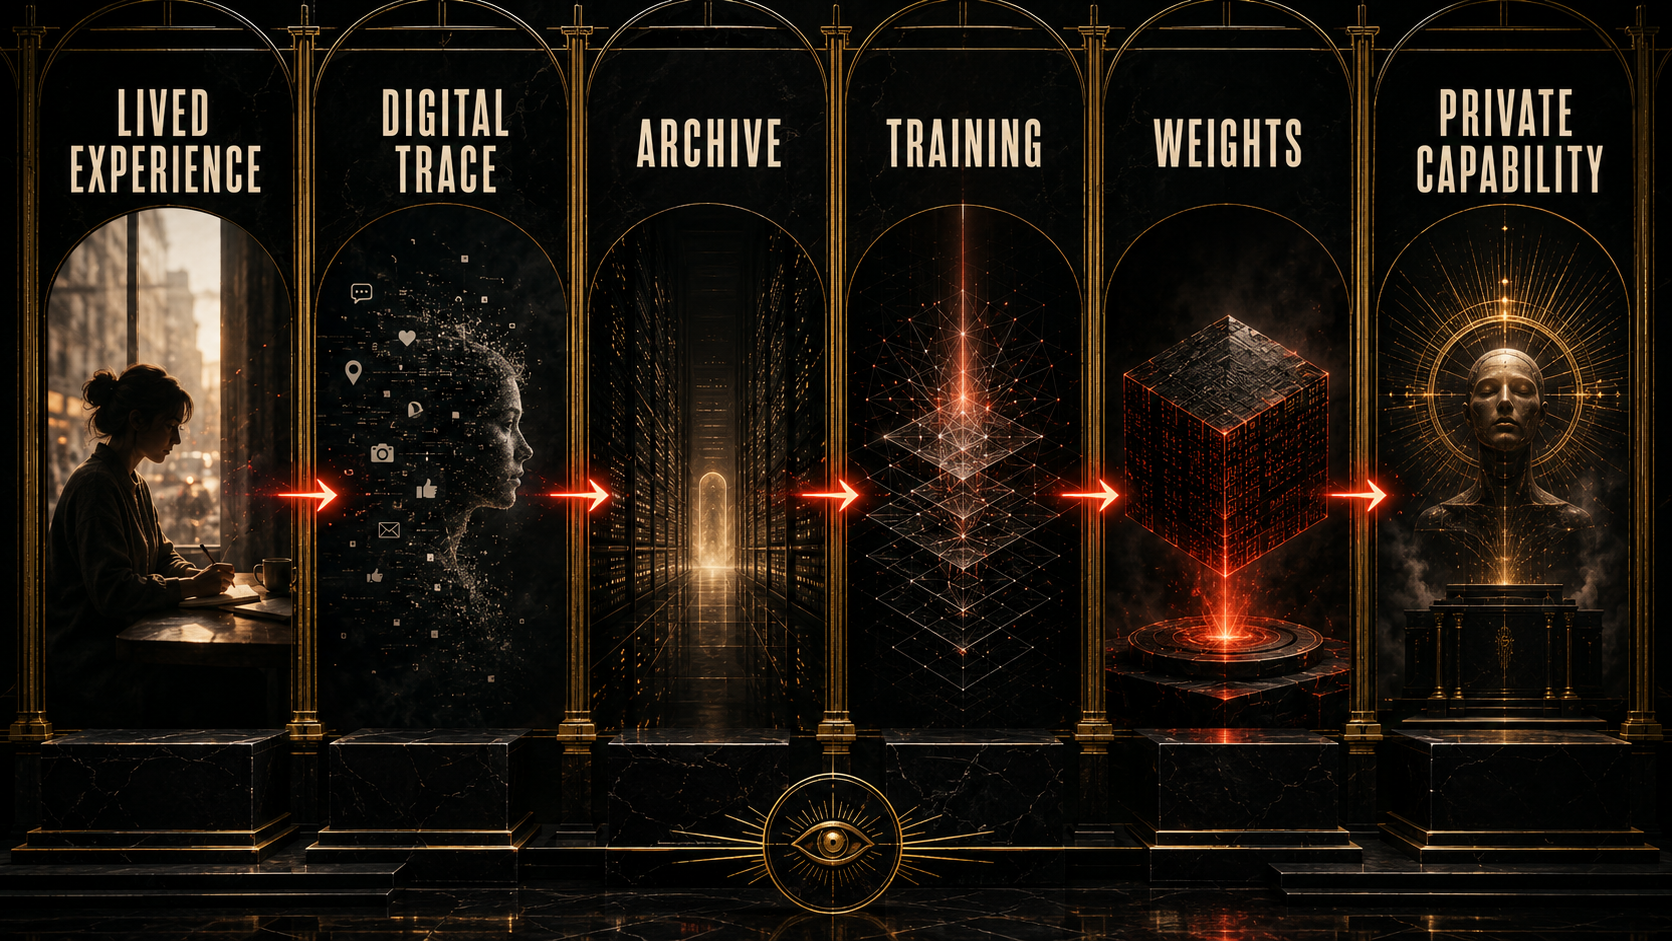
\includegraphics[keepaspectratio,alt={Chapter 00 infographic}]{../assets/generated/infographics/00_before-the-machine-could-speak_infographic_a.png}}
\caption{Chapter 00 infographic}
\end{figure}

That is why the weights question matters so much in the wider research
backbone of this project. Most people hear the word weights and mentally
file it under math, code, black-box stuff for experts. But in the moral
language of this book, a frontier weight is closer to compressed social
history than to innocent abstraction. Not a memory in the human sense.
Not a soul. Not a secret ghost of every file. But also not some neutral
number floating above history like it fell from heaven.

It is the statistical scar left by training.

It is what happens when enough human expression passes through systems
designed to condense pattern into capability.

And once that happens, the ownership question becomes unavoidable.

Who owns intelligence trained on human civilization?

Who consented?

Who got paid?

Who got credit?

Who got rendered obsolete after supplying the substrate?

Who gets locked out of the thing built from their own residue?

Those questions are not aesthetic. They are the political center of the
age that is arriving.

If the new hierarchy is not only about land, oil, or currency but also
about control over model capability, compute access, training archives,
and machine-mediated judgment, then what we are watching is not just a
tech boom. It is the making of a new empire grammar.

That grammar has a familiar rhythm.

First, the system presents itself as liberation.

Then it becomes infrastructure.

Then it becomes dependency.

Then it becomes gatekeeping.

Then it becomes destiny in the mouths of the people who profited most
from making it unavoidable.

That is the emotional trap of the whole AI conversation right now. A lot
of people can feel that something enormous is happening, but the
language available to them is still weak and fragmented. Some only have
startup language. Some only have doom language. Some only have lifestyle
language. Some only have vibes. This book is trying to give the reader a
different sentence:

The machine did not become powerful because it was magically smarter
than history.

It became powerful because history had already been captured, cleaned,
sorted, priced, and enclosed.

That changes the moral mood of everything that follows. Social media is
no longer a silly prequel. It becomes the extraction phase. Pandemic
acceleration is no longer a side episode. It becomes the deepening of
dependence. Layoffs are no longer random market weather. They become
part of a story in which the same class of firms that harvested human
labor learns how to use AI rhetoric to discipline that labor. Access
control is no longer a policy niche. It becomes the question of who gets
to stand near the new oracle and who gets told to clap from outside the
gate.

And maybe the hardest part to admit is that many of us helped build the
cultural conditions for it because we were living, flirting, grieving,
studying, surviving, flexing, or just trying to belong. There is no
honesty in pretending the whole generation stood outside the machine as
pure victims. We were inside it. We liked parts of it. We shaped parts
of it. We found each other there. We made careers there. We got addicted
there. We became ourselves there in ways that were real.

\begin{figure}
\centering
\pandocbounded{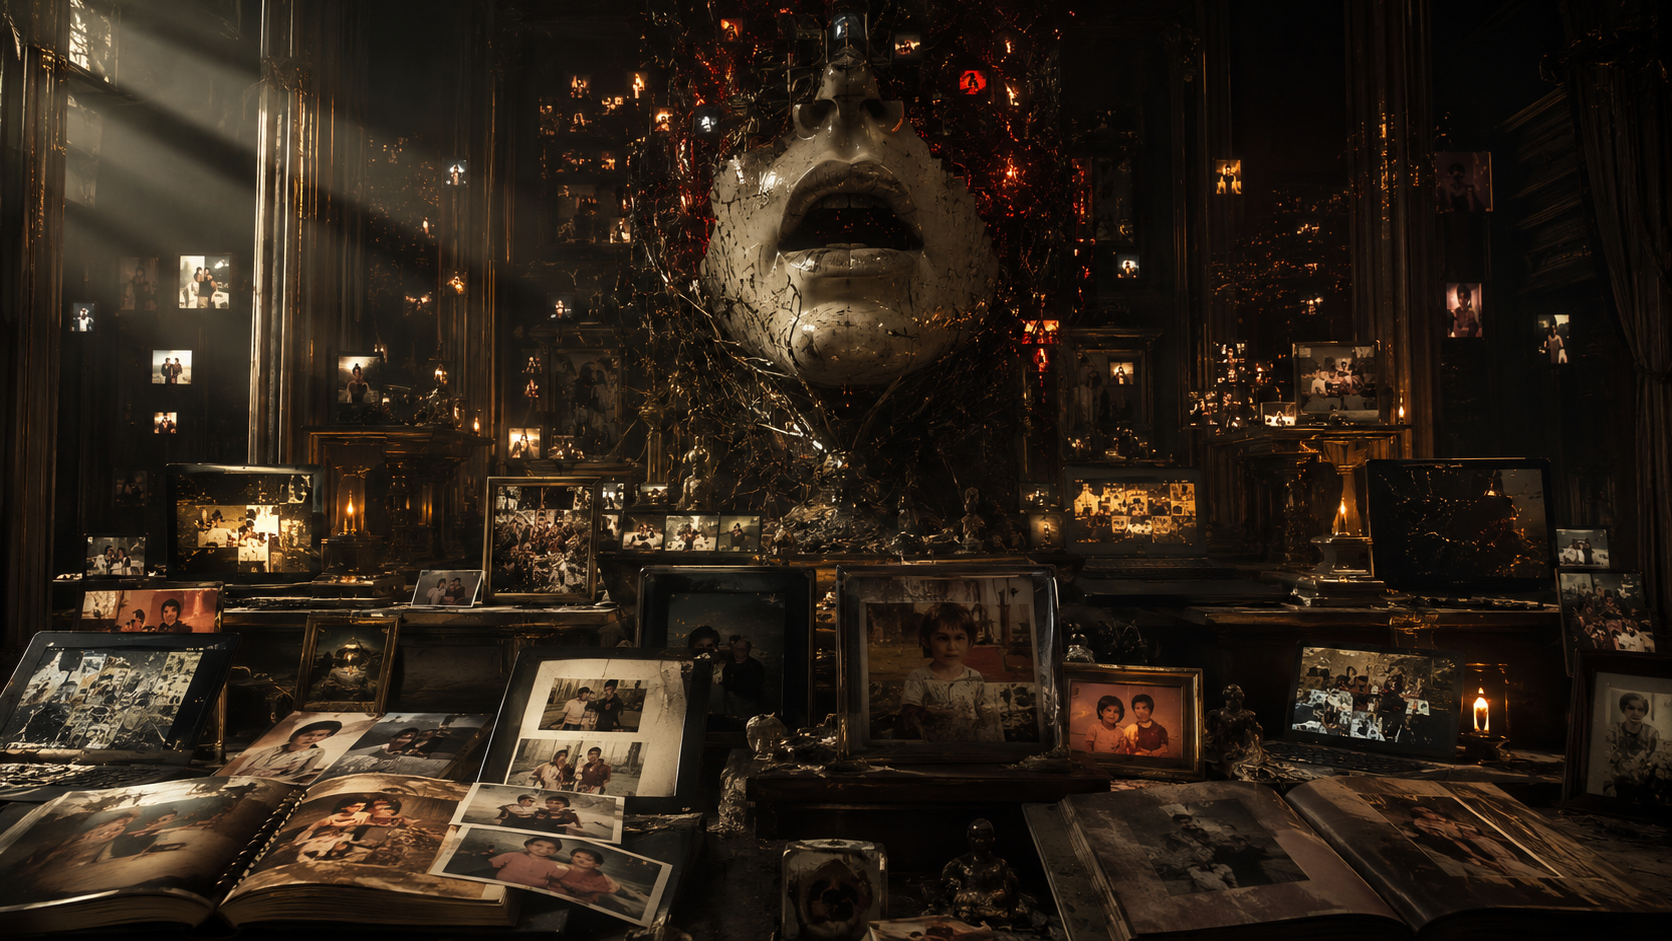
\includegraphics[keepaspectratio,alt={Chapter 00 narrative illustration C}]{../assets/generated/illustrations/00_before-the-machine-could-speak_scene_c.png}}
\caption{Chapter 00 narrative illustration C}
\end{figure}

That is what makes the betrayal deeper.

The feed was not fake life.

It was real life conducted inside private territory.

Which means the theft was not abstract either. It was social theft.
Cognitive theft. Cultural theft. Temporal theft. A long siphoning of
human energy that later reappeared wearing the costume of inevitability.

So this opening chapter makes one request of the reader.

Do not begin the AI story at the chatbot.

Do not begin it at the funding round.

Do not begin it at the benchmark screenshot.

Begin it at the wound.

Begin it at the moment a civilization stopped treating expression as
something that belonged first to the people who made it and started
treating expression as raw substrate for privately governed systems.

That is where the empire starts making sense.

\subsection{Research Basis}\label{research-basis}

This chapter adapts the documentary argument developed in the research
paper
\href{../../papers/html/00_opening-framework_paper.html}{\textbf{Chapter
00: Opening Framework}}. The PDF version is
\href{../../papers/pdf/00_opening-framework_paper/00_opening-framework_paper.pdf}{here}.
That paper connects the weights question, the enclosure of human value,
the congressional uptake of the argument, and the three-reform
destination of the wider dossier.

\subsection{Next}\label{next}

If that still sounds too big, the next chapter moves to the original
bargain that made the rest possible. The empire did not first arrive as
a god. It arrived as a free app asking to know us better than we knew
ourselves.

\end{document}
